\chapter{Results}\label{cha:Results}

\textit{Pure facts and as objectively as possible. Don't analyze, comment or evaluate.  If describe implementation process, only describe largest decisions.}


\section{System overview}\label{sec:res:sys}

Describe the system as a whole here, and what parts have been done.

\begin{enumerate}
    \item Reader module (inläsningsmodul, name????)
    \item Input module (indata) name???
    \item Output module (utdata)
    \item Purchase history db
    \item Product data db
    \item Parameters??? Or will we ignore this for the thesis work?
    \item Algorithm
    \item Control programs (But it's really just modifications of the algorithms)
    \item General/Personalized/Related recommendations db
    \item Remote API
    \item Web shop
    \item Admin web API?
\end{enumerate}

\Warning[TODO]{ Need a figure which describes the different parts }


\subsection{Input module}\label{sec:res:input}

Describe plugin based architecture here.

Add plugin scripts to:


\begin{lstlisting}
    lib/reader_plugins
\end{lstlisting}

Basic look is:

% TODO include files instead, or delegate to appendix?
\begin{lstlisting}[language=python]
class MyPlugin():

    def add_arguments(self, parser):
        """Parse command line arguments"""

        parser.description = "Load plugin data"

        parser.add_argument('data_file', metavar='data_file', type=str,
                            help='the file to parse')

    def load(self, args):
        """Load users and products."""

        products = {}
        users = {}

        # Parse data file
        with open(args.data_file) as csvfile:
            reader = csv.DictReader(csvfile, delimiter=';', quoting=csv.QUOTE_NONE)

            for row in reader:
                user_id = row['shopper_id']
                isbn = row['isbn']
                title = row['description']

                if user_id not in users:
                    users[user_id] = User(user_id)

                if isbn not in products:
                    product = Product(isbn)
                    product.isbn = isbn
                    product.title = title
                    products[isbn] = product

                users[user_id].add_history(isbn, 1)

        return users, products
\end{lstlisting}

An example plugin is described in appendix X. \Warning[TODO]{ Make it happen! }

Can describe how to dynamically locate modules with python, but that's not the purpose is it? Just describe that it can be done I guess?




\section{Data}

The available datasets are described in detail in \appendixref{cha:datasets}. All data will in unweighted binary form \eqref{eq:hist}.

An alternative to unweighted binary data is weighted data, where $h_{u, i} = x$ means that user $u$ has interacted with item $i$ $x$ times. There is some support in the available datasets (\textit{alpha}, \textit{alpha2}) but most of the datasets does not, which is why the focus is on datasets in unweighted binary form.

Another popular format is ratings, which \textit{movielens1m} is derived from. Generating recommendations with explicit feedback, such as ratings, is well researched but fundamentally different from implicit feedback systems. The focus on this thesis is recommendations for implicit feedback systems which is why ratings are not considered in their raw form.

During supervised learning the datasets will be divided into training, validation and test sets with a ratio of 70\%, 15\% and 15\% respectively. When a validation set is not necessary, it will be ignored and only the training and test sets will be used. Alternatively a new split with only training and test sets could be used with, for example, a split of 80\% and 20\% could be used. This thesis uses the same approach because of simplicity, there's no need to track different kinds of splits for the same data.

As mentioned in \sectionref{sec:background:theory:suplearn} there are different ratios commonly used to split datasets. There is no ratio which is always the best, they depend on the amount of data available, the modeled domain and the algorithms chosen. A split of 70/15/15 was chosen uniformly for simplicity reasons.





\newpage


\section{Data}

The available datasets are described in detail in \appendixref{cha:datasets}. All data will in unweighted binary form \eqref{eq:hist}.

An alternative to unweighted binary data is weighted data, where $h_{u, i} = x$ means that user $u$ has interacted with item $i$ $x$ times. There is some support in the available datasets (\textit{alpha}, \textit{alpha2}) but most of the datasets does not, which is why the focus is on datasets in unweighted binary form.

Another popular format is ratings, which \textit{movielens1m} is derived from. Generating recommendations with explicit feedback, such as ratings, is well researched but fundamentally different from implicit feedback systems. The focus on this thesis is recommendations for implicit feedback systems which is why ratings are not considered in their raw form.

During supervised learning the datasets will be divided into training, validation and test sets with a ratio of 70\%, 15\% and 15\% respectively. When a validation set is not necessary, it will be ignored and only the training and test sets will be used. Alternatively a new split with only training and test sets could be used with, for example, a split of 80\% and 20\% could be used. This thesis uses the same approach because of simplicity, there's no need to track different kinds of splits for the same data.

As mentioned in \sectionref{sec:background:theory:suplearn} there are different ratios commonly used to split datasets. There is no ratio which is always the best, they depend on the amount of data available, the modeled domain and the algorithms chosen. A split of 70/15/15 was chosen uniformly for simplicity reasons.



\newpage




\section{Training curves}\label{sec:graphs:training_curves}

Both \textit{katz-eig} and \textit{link-analysis} are iterative algorithms. Their descriptions use the phrase ``repeat until convergence''.  With training curves, which plots the evaluation metric with the respect to epochs, the number of iterations, the effect of running more iterations can be seen.

Each $K$ are different for each dataset, see \appendixref{app:opt_params}, and $beta = \frac{1}{\|A_{train}\|_2}$.

\subsection{katz-eig}

\FloatBarrier

\twodiffpic{fig/katzeig_t/alphaS_katzeig_t.png}{\textit{alphaS}}
{fig/katzeig_t/eswc2015movies_katzeig_t.png}{\textit{eswc2015movies}}

\twodiffpic{fig/katzeig_t/movielens_katzeig_t.png}{\textit{movielens1m}}
{fig/katzeig_t/romeo_katzeig_t.png}{\textit{romeo}}

\FloatBarrier

The jagged line represents $\|S_t - S_{t - 1}\|_2$, which is a measure of the difference between the current iteration $t$ and the previous iteration. This was made as a measure of the convergence criteria. Convergence was reached with relatively few iterations, but the matrix $S$ is small and the calculation has low complexity.

In all following usages of \textit{katz-eig}, a value of $\epsilon = 0.01$ was used to break iterations if $\|S_t - S_{t - 1}\|_2 < \epsilon$.

\newpage


\subsection{link-analysis}

Each $\gamma$ and $\eta$ are different for each dataset, see \appendixref{app:opt_params}.

\twodiffpic{fig/link_t/alphaS_link_t.png}{\textit{alphaS}}
{fig/link_t/eswc2015books_link_t.png}{\textit{eswc2015books}}

\twodiffpic{fig/link_t/movielens1m_link_t.png}{\textit{movielens1m}}
{fig/link_t/romeo_link_t.png}{\textit{romeo}}

\Warning[TODO]{ More plots }

For \textit{link-analysis} convergence is also fast. The choice here was to fix $t_{max}$ to a fixed value instead of measuring convergence either by calculating $\| \PR_t - \PR_{t - 1} \|_2$
or by explicitly calculating \textit{F-measure} and measuring the change. This was done because the iteration step in \textit{link-analysis}, in contrast to \textit{katz-eig}, handles large matrices and calculations such as these would be time consuming.

In all following usages of \textit{link-analysis}, the iteration count was fixed to $t_{max} = 3$.


\newpage


\section{Learning curves}\label{sec:graphs:learning_curves}

Learning curves plots the evaluation metric with respect to a varying training set size. The expectation here is that the algorithms should fit better the bigger the training set size becomes, given the same test set. The algorithms should produce better recommendations the more data they have to learn from. Learning curves is a good way to see if the algorithms work like they're supposed to.

The evaluation uses the training matrix $A_{train}$ and the test set matrix $A_{test}$. For each step a random selection of a specific size is selected from $A_{train}$, recommendations are generated and evaluated against the same test set $A_{test}$. The dimensions of the matrices will the same, only the number of non-zero elements are increased with the training set size. This was done 10 times for each training set size as to remove variations from the random selection. The evaluation metric used was \textit{F-measure} with top-10 recommendations.

Optimized parameters as described in \tableref{tab:katzeig_params_used} and \tableref{tab:linkanalysis_params_used} were used.

\twopic{fig/learning_curves/alphaS_learning_perf.png}{fig/learning_curves/alphaS_learning_time.png}{
\textit{alphaS}
}
\twopic{fig/learning_curves/eswc2015books_learning_perf.png}{fig/learning_curves/eswc2015books_learning_time.png}{
\textit{eswc2015books}
}
\twopic{fig/learning_curves/movielens_learning_perf.png}{fig/learning_curves/movielens_learning_time.png}{
\textit{movielens1m}
}
\twopic{fig/learning_curves/romeo_learning_perf.png}{fig/learning_curves/romeo_learning_time.png}{
\textit{romeo}
}

A notable observation about the runtime is that the runtime for \textit{link-analysis} increases almost linearly with the increase in training set size, the runtime for \textit{katz-eig} is almost indifferent. This is to be expected as \textit{katz-eig} operates on a low-rank approximation of the interaction matrix $A_{train}$ while \textit{link-analysis} operates directly on the matrix. The sparse matrix format (\sectionref{sec:background:theory:matrix}) which discards zero elements during calculations is computationally more complex as the sparsity decreases.

\FloatBarrier

\newpage



\section{Parameter analysis}\label{sec:parameters}

\textit{How do the parameter space look?}


\subsection{katz-eig}

There are two parameters to \textit{katz-eig}: $\beta$, the link diminishing factor and $K$ specifying the $K$-rank approximation. $\beta$ is a continous value satisfying $0 < \beta \leq \frac{1}{\|A_{train}\|_2}$. If $\beta = 0$ then the algorithm will only output 0 and if $\beta > \frac{1}{\|A_{train}\|_2}$ the iterations will not converge. $K > 0$ is a discrete value.

What follows is plots over both of the parameters $K$ and $\beta$. The plots are evaluated using \textit{F-measure} w.r.t. the test set using top-10 recommendations.

\begin{figure}[h!]
\centering
\begin{minipage}{.5\textwidth}
    \centering
    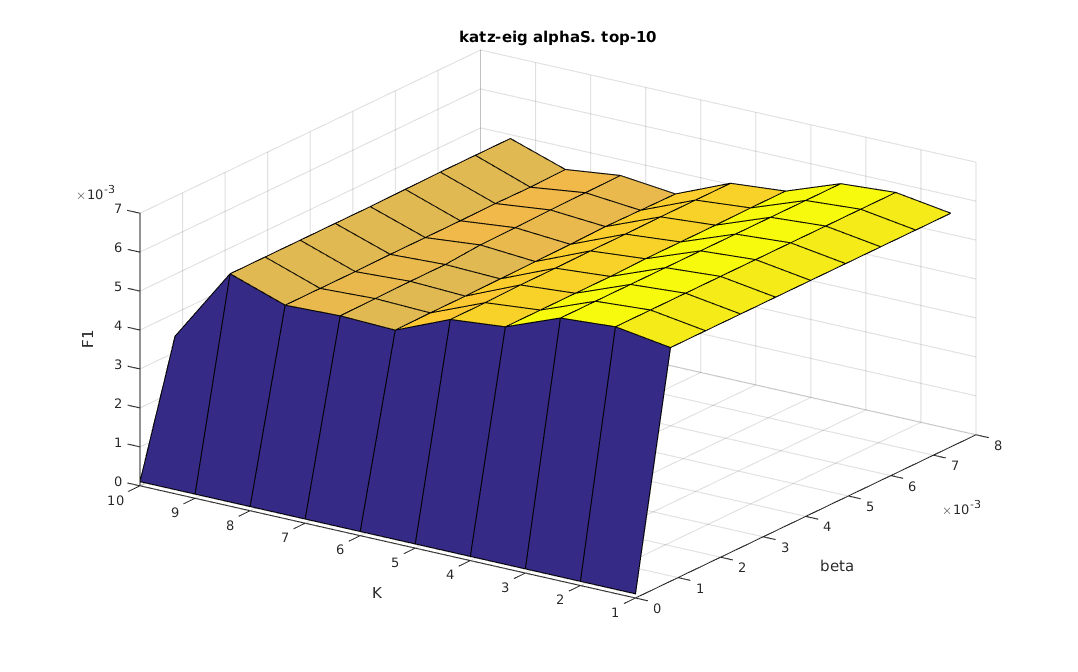
\includegraphics[width=\linewidth]{fig/katzeig_beta_k/alphaS_katzeig.png}
    \captionof{figure}{\textit{alphaS}}
\end{minipage}%
\begin{minipage}{.5\textwidth}
    \centering
    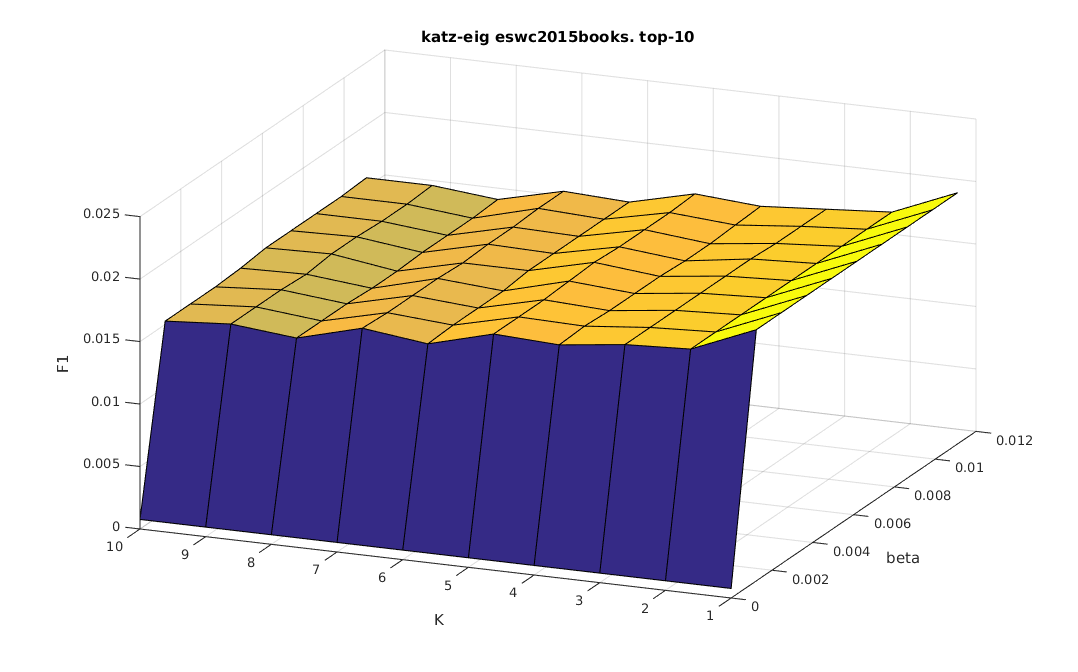
\includegraphics[width=\linewidth]{fig/katzeig_beta_k/eswc2015books_katzeig.png}
    \captionof{figure}{\textit{eswc2015books}}
\end{minipage}
\end{figure}

\begin{figure}[h!]
\centering
\begin{minipage}{.5\textwidth}
    \centering
    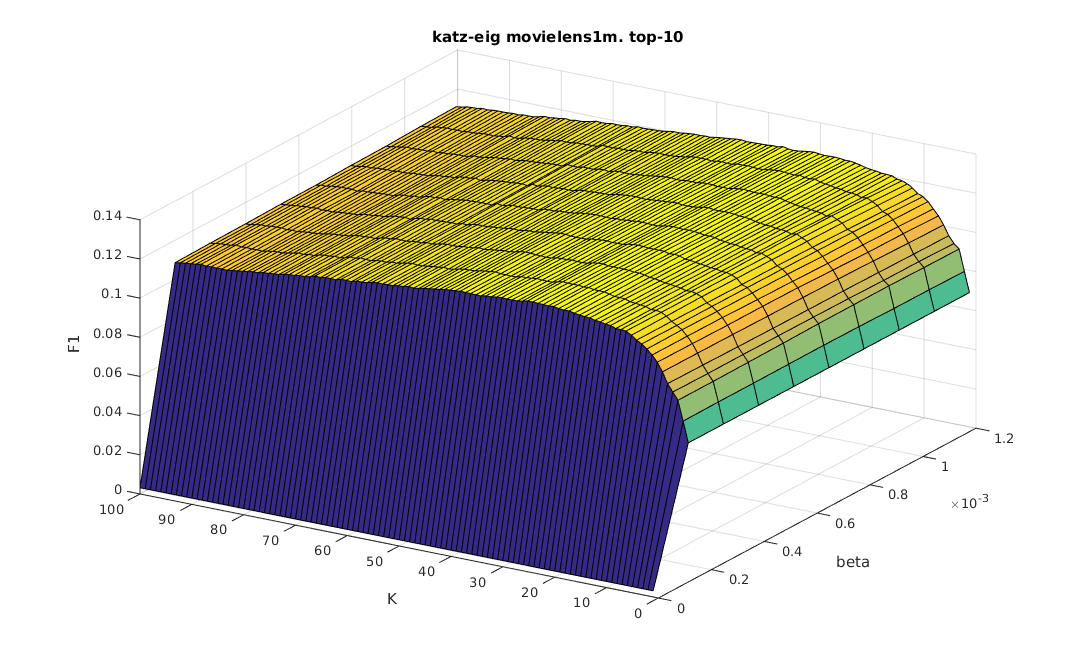
\includegraphics[width=\linewidth]{fig/katzeig_beta_k/movielens_katzeig.png}
    \captionof{figure}{\textit{movielens1m}}
\end{minipage}%
\begin{minipage}{.5\textwidth}
    \centering
    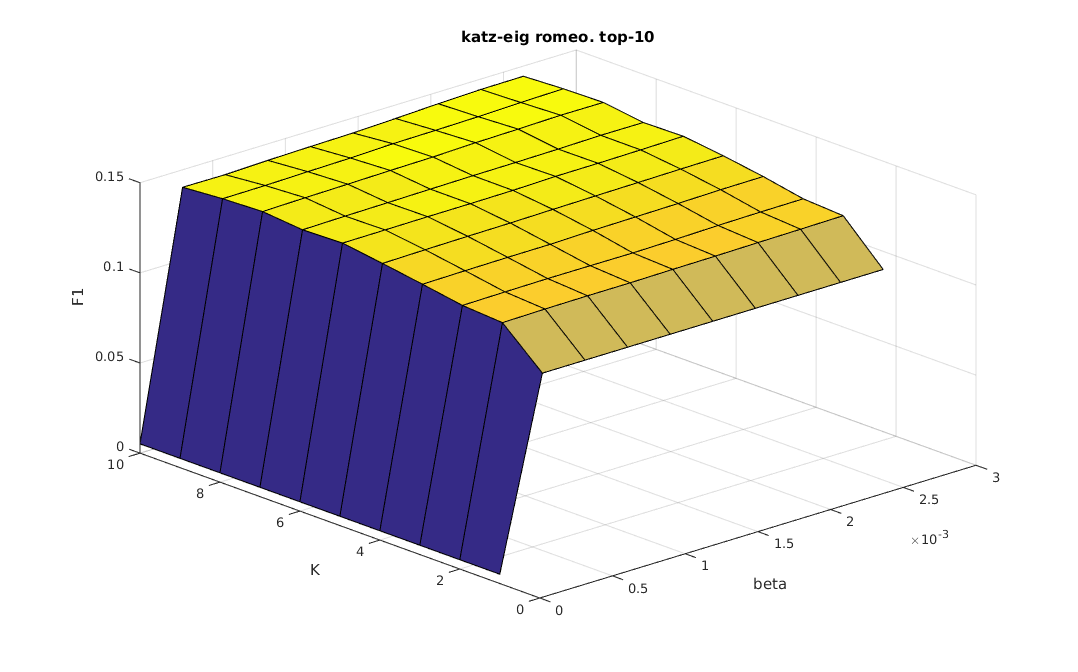
\includegraphics[width=\linewidth]{fig/katzeig_beta_k/romeo_katzeig.png}
    \captionof{figure}{\textit{romeo}}
\end{minipage}
\end{figure}




It seems like $beta$ doesn't have a very big impact on the function value. Some plots with a fixed $K$ follows to better see differences.

The range examined is $0 < \beta \leq \beta_{max} = \frac{1}{\|A_{train}\|_2}$ with a $K$ selected to fit the specific dataset. Again evaluated using \textit{Precision}, \textit{Recall} and \textit{F-measure} w.r.t. the test set using the top-10 recommendations.

\FloatBarrier

\begin{figure}[h!]
\centering
\begin{minipage}{.5\textwidth}
    \centering
    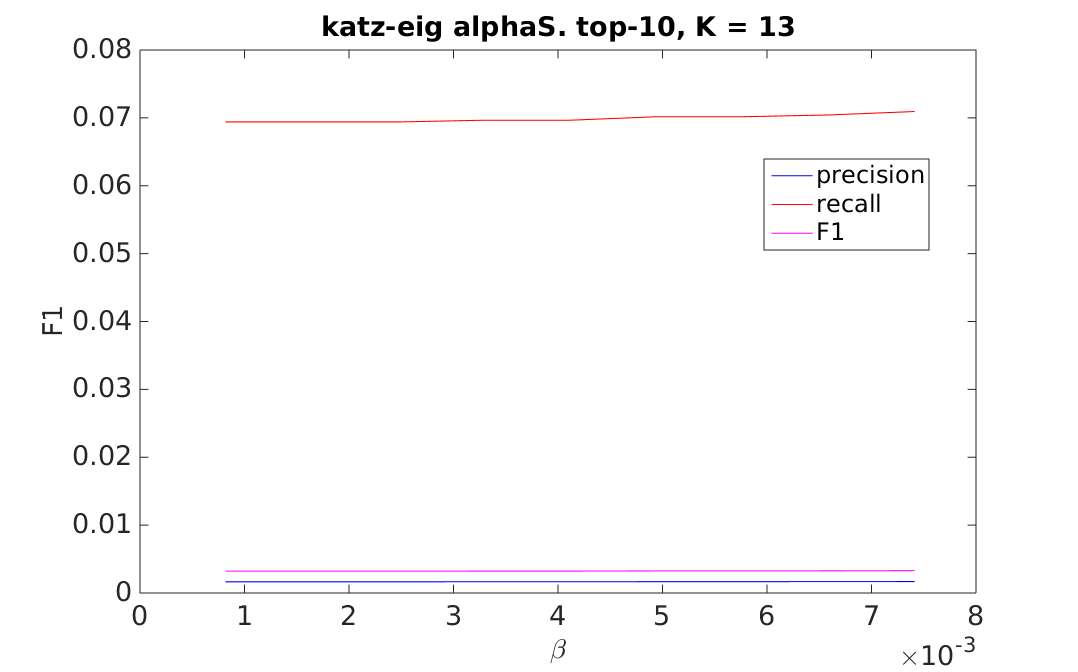
\includegraphics[width=\linewidth]{fig/katzeig_beta/alphaS_katzeig_beta.png}
    \captionof{figure}{\textit{alphaS}.
        $\beta_{max}$ is the best value with a $1.9\%$ diff between the minimum and the maximum \textit{F1} value.}
\end{minipage}%
\begin{minipage}{.5\textwidth}
    \centering
    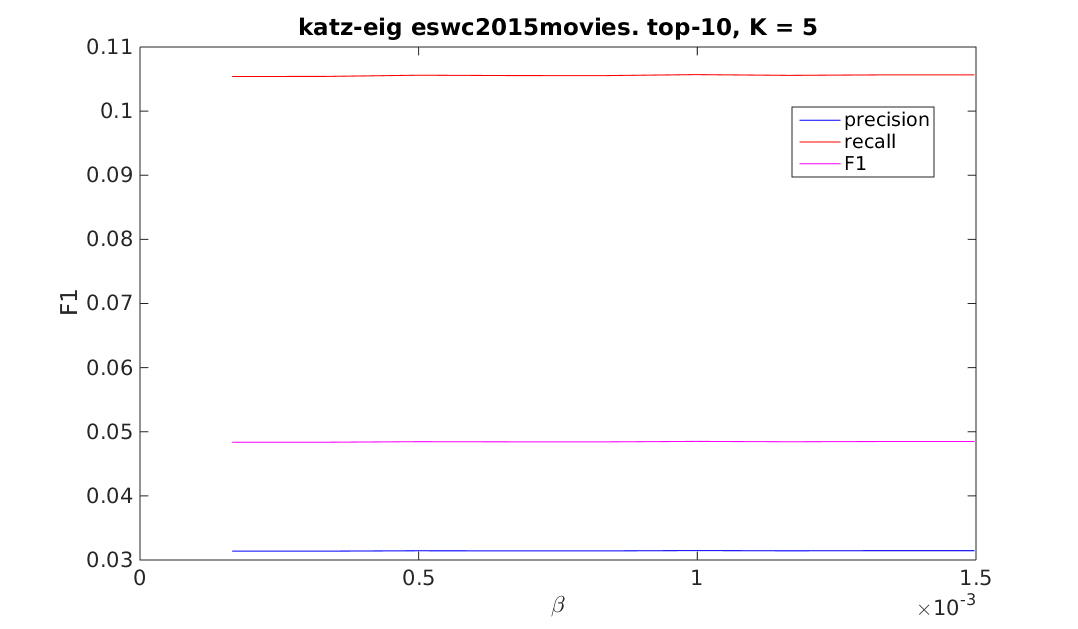
\includegraphics[width=\linewidth]{fig/katzeig_beta/eswc2015movies_katzeig_beta.png}
    \captionof{figure}{\textit{eswc2015movies}.
        $\beta_{max}$ is not the best value with a $0.3\%$ diff between the minimum and the maximum \textit{F1} value.}
\end{minipage}
\end{figure}

\begin{figure}[h!]
\centering
\begin{minipage}{.5\textwidth}
    \centering
    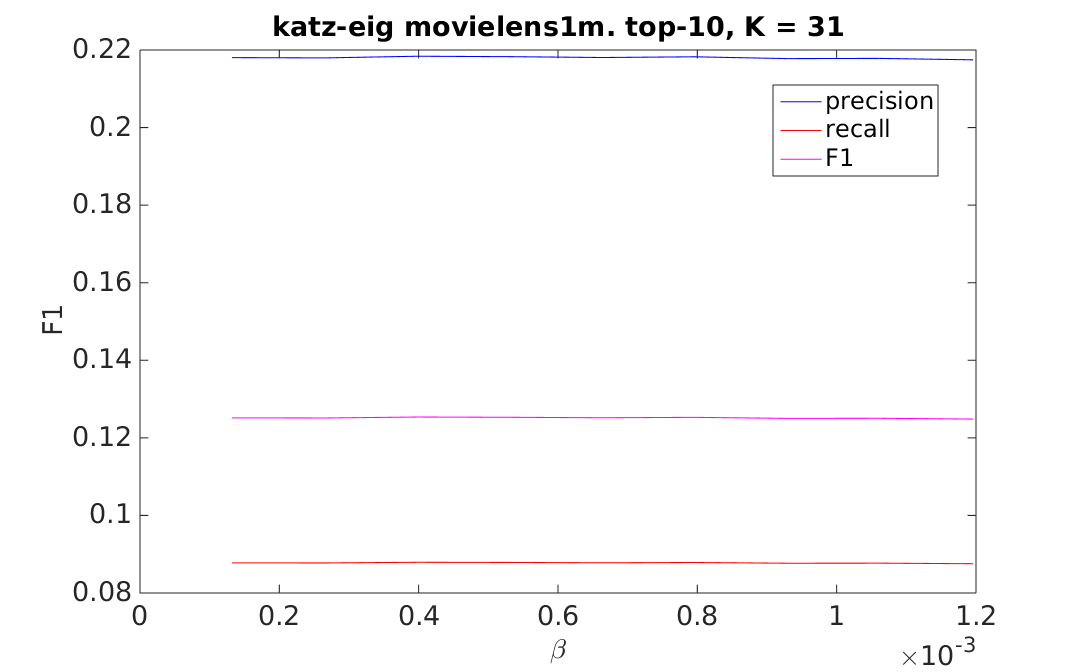
\includegraphics[width=\linewidth]{fig/katzeig_beta/movielens_katzeig_beta.png}
    \captionof{figure}{\textit{movielens1m}.
        $\beta_{max}$ is not the best value with a $0.41\%$ diff between the minimum and the maximum \textit{F1} value.}
\end{minipage}%
\begin{minipage}{.5\textwidth}
    \centering
    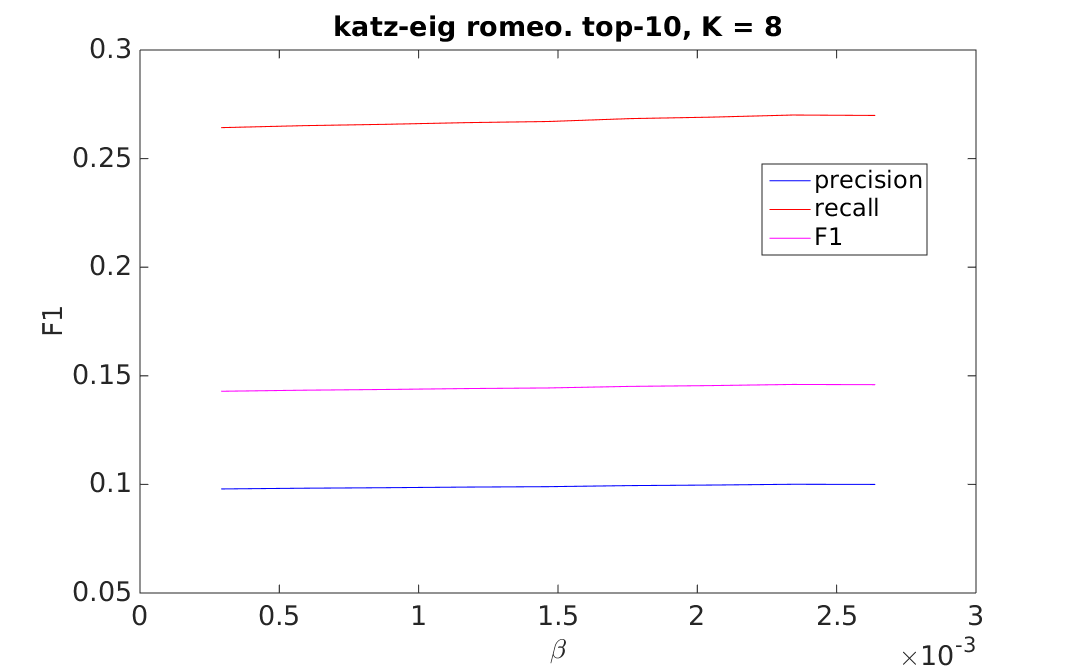
\includegraphics[width=\linewidth]{fig/katzeig_beta/romeo_katzeig_beta.png}
    \captionof{figure}{\textit{movielens1m}.
        $\beta_{max}$ is not the best value with a $2.09\%$ diff between the minimum and the maximum \textit{F1} value.}
\end{minipage}
\end{figure}

\FloatBarrier

The difference between the optimal $\beta$ and an arbitrary selected $\beta$ isn't very large. Even smaller is the difference between the optimal $\beta$ and $\beta_{max}$.  \Tableref{tab:katzeig_beta} is a summary of the evaluated values.

\begin{table}[h!]
    \centering
    \begin{tabular}{| c | r | r | r | r | l |}
        \hline
        \textbf{dataset}        & \textbf{diff between $\beta_{opt}$ and $\beta_{max}$ }    & \textbf{diff between $f_{min}$ and $f_{max}$} \\ \hline

        \textit{alphaS}         & 0~\%      & 2.0~\%    \\ \hline
        \textit{eswc2015books}  & 0~\%      & 0\%       \\ \hline
        \textit{eswc2015movies} & 0.039~\%  & 0.28~\%   \\ \hline
        \textit{movielens1m}    & 0.41~\%   & 0.41~\%   \\ \hline
        \textit{romeo}          & 0.072~\%  & 2.1~\%    \\ \hline


    \end{tabular}
    \caption{A summary of evaluating different $\beta$. $\beta_{max} = \frac{1}{\|A_{train}\|_2}$ is the maximally examined $\beta$ and $\beta_{opt}$ is the optimal $\beta$ found in the range $0 < \beta \leq \beta_{max}$. $K$ is individually optimized for the different datasets. $f_{min}$ and $f_{max}$ are the minimal and maximal \textit{F1} values obtained.}
    \label{tab:katzeig_beta}
\end{table}

\FloatBarrier

\newpage


The $K$-rank approximation represents different available models for \textit{katz-eig}. The following plots show different values of $K$, evaluated w.r.t. the test set. $\beta = \frac{1}{\|A_{train}\|}_2$ for all datasets. $K_{m}$ is the value of $K$ which gives the best \textit{F-measure} for each dataset.

\FloatBarrier

\begin{figure}[h!]
\centering
\begin{minipage}{.5\textwidth}
    \centering
    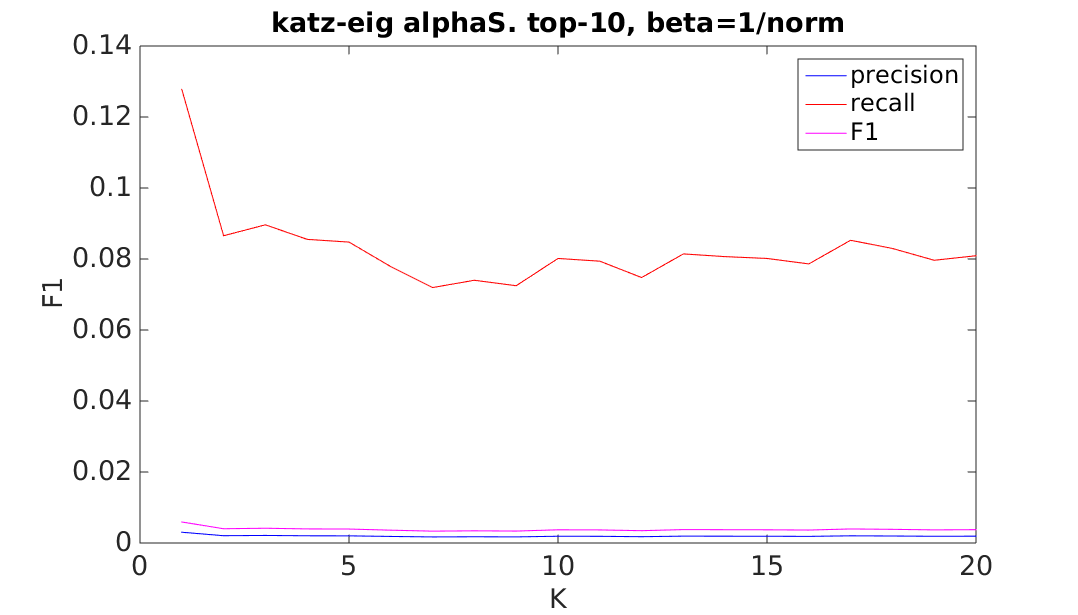
\includegraphics[width=\linewidth]{fig/katzeig_k/alphaS_katzeig_K.png}
    \captionof{figure}{\textit{alphaS} $K_{m} = 13$}
\end{minipage}%
\begin{minipage}{.5\textwidth}
    \centering
    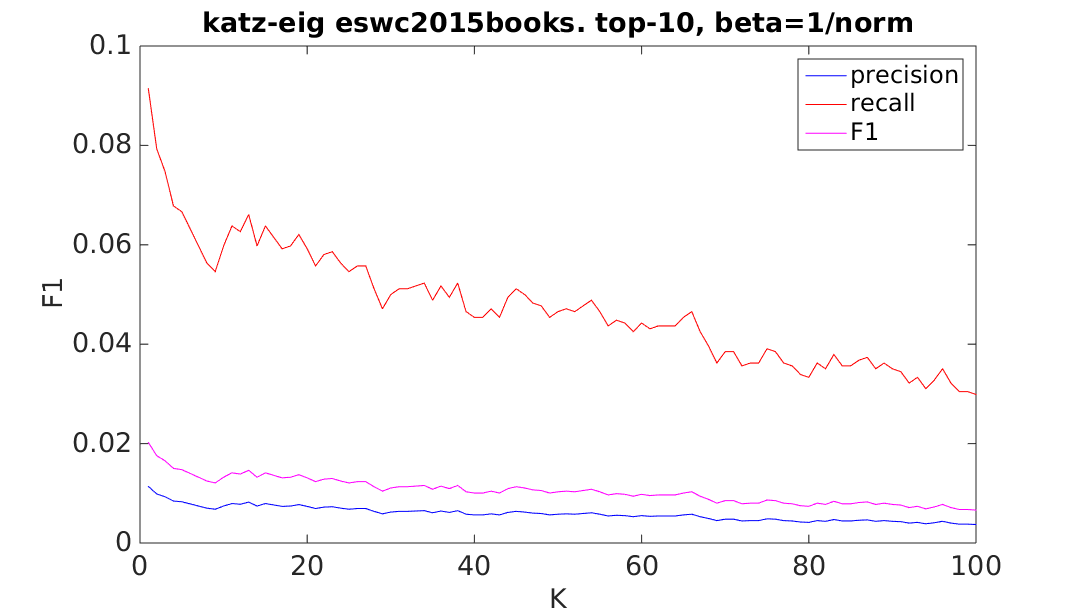
\includegraphics[width=\linewidth]{fig/katzeig_k/eswc2015books_katzeig_K.png}
    \captionof{figure}{\textit{eswc2015books} $K_{m} = 1$}
\end{minipage}
\end{figure}

\begin{figure}[h!]
\centering
\begin{minipage}{.5\textwidth}
    \centering
    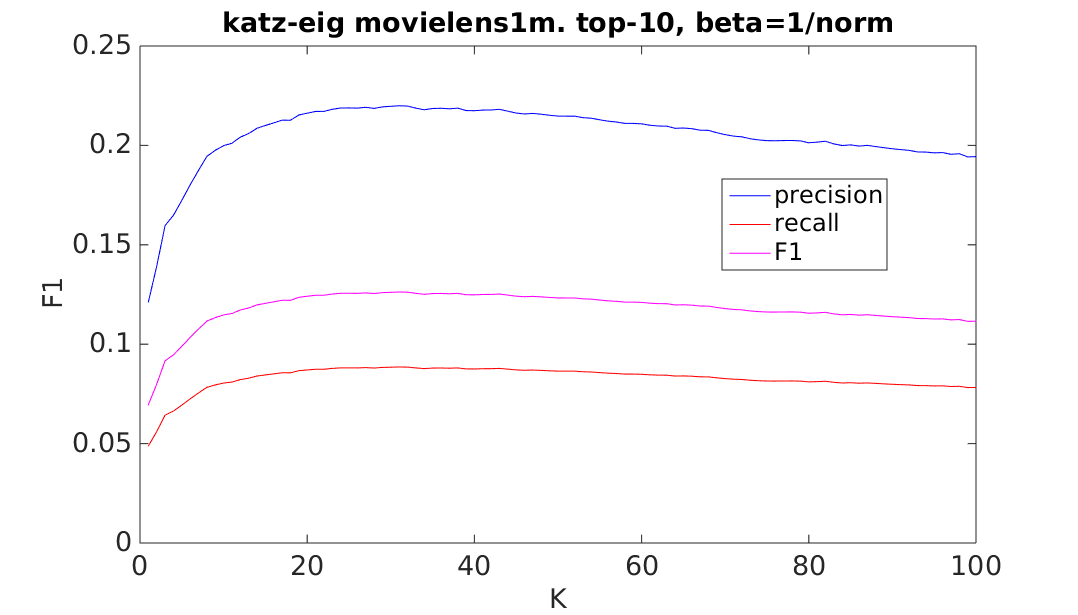
\includegraphics[width=\linewidth]{fig/katzeig_k/movielens_katzeig_K.png}
    \captionof{figure}{\textit{movielens1m} $K_{m} = 31$}
\end{minipage}%
\begin{minipage}{.5\textwidth}
    \centering
    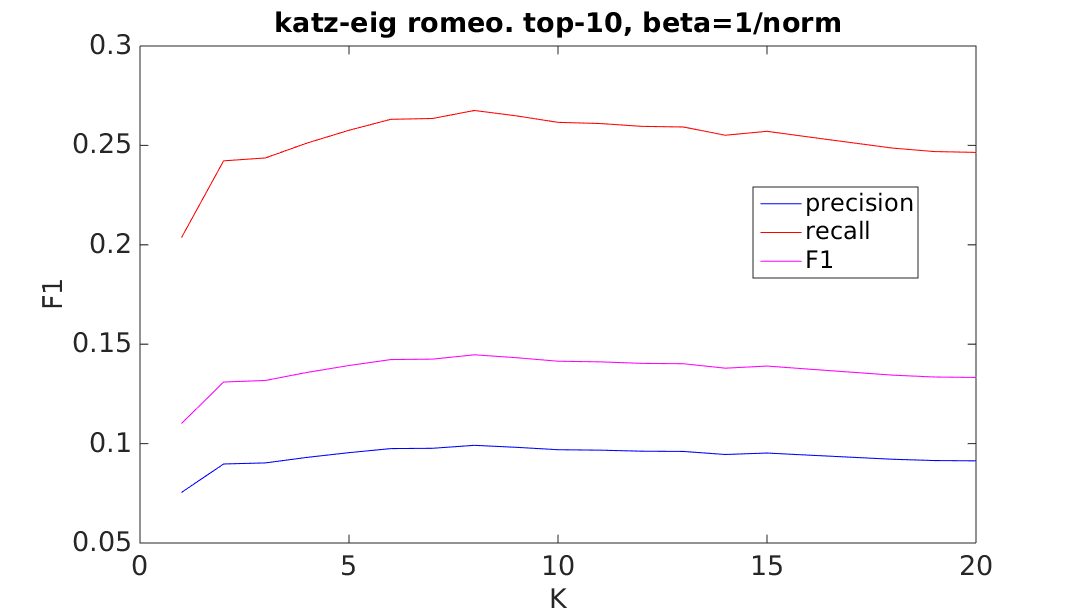
\includegraphics[width=\linewidth]{fig/katzeig_k/romeo_katzeig_K.png}
    \captionof{figure}{\textit{romeo} $K_{m} = 8$}
\end{minipage}
\end{figure}

\Warning[TODO]{ Plot of \textit{eswc2015movies}? }

%\begin{figure}[h!]
%\centering
%\begin{minipage}{.5\textwidth}
    %\centering
    %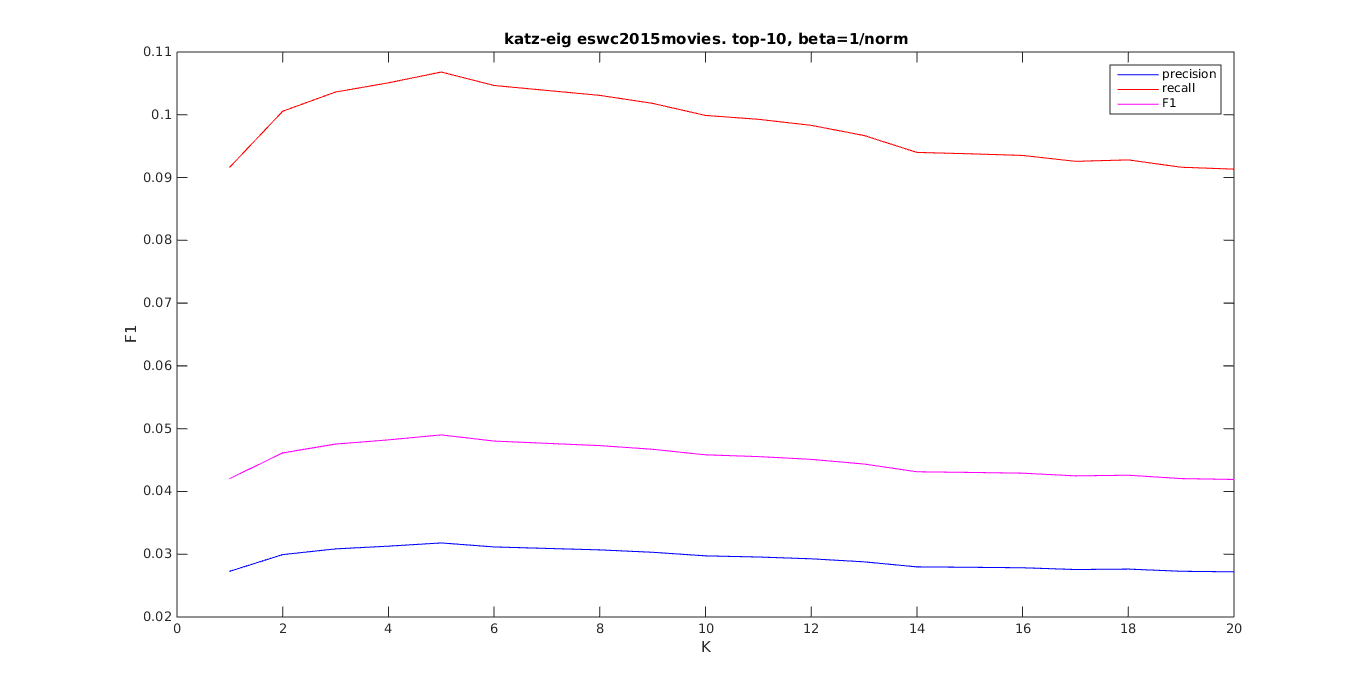
\includegraphics[width=\linewidth]{fig/katzeig_k/eswc2015movies_katzeig_K.png}
    %\captionof{figure}{\textit{eswc2015movies} $K_{m} = 5$}
%\end{minipage}%
%\begin{minipage}{.5\textwidth}
    %\centering
    %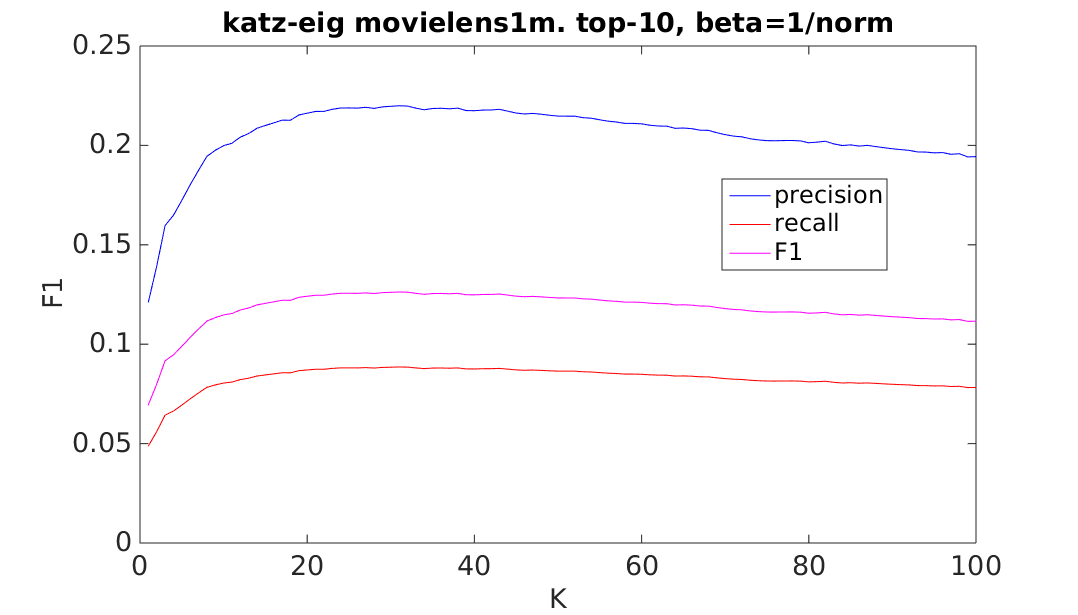
\includegraphics[width=\linewidth]{fig/katzeig_k/movielens_katzeig_K.png}
    %\captionof{figure}{\textit{movielens1m} $K_{m} = 31$}
%\end{minipage}
%\end{figure}

%\begin{figure}[h!]
%%\centering
%\begin{minipage}{.5\textwidth}
    %%\centering
    %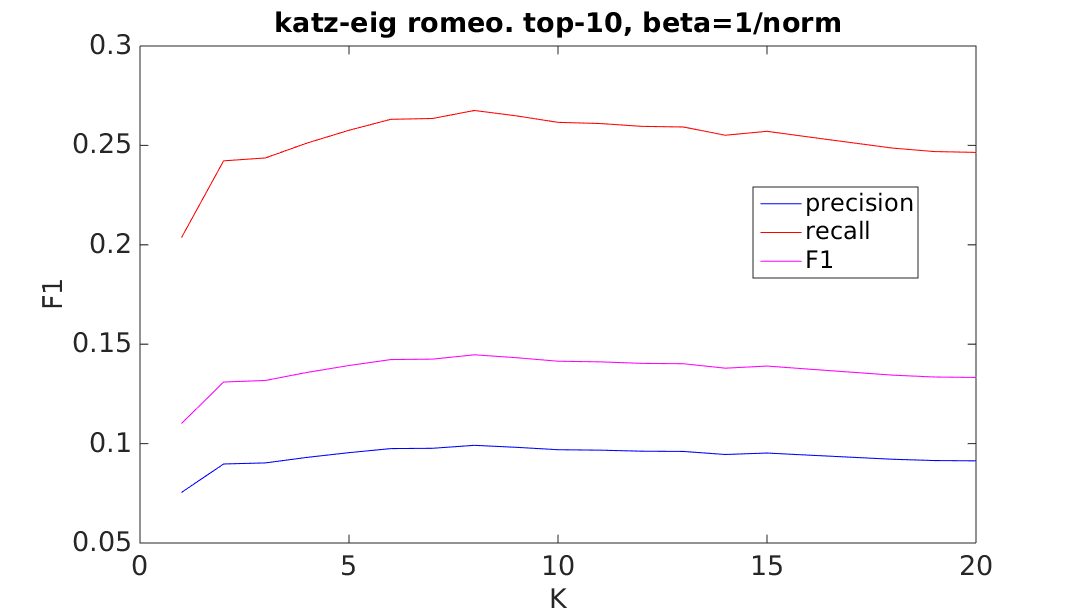
\includegraphics[width=\linewidth]{fig/katzeig_k/romeo_katzeig_K.png}
    %\captionof{figure}{\textit{romeo} $K_{m} = 8$}
%\end{minipage}%
%\end{figure}

\FloatBarrier

The function space w.r.t. $K$ is fairly smooth if not entirely convex. \textit{eswc2015books} is an outlier with a low optimal value $K = 1$ and many local optima. The other datasets display more smooth functions, but there are clear local optima with both \textit{alphaS} and \textit{romeo}.

Also of note is that the functions start to decline at different $K$. \textit{eswc2015movies} declines already at $K = 5$ but it's only at around $K = 30$ \textit{movielens1m} starts to decline. As noted earlier \textit{eswc2015books} has it's optima already at $K = 1$.


\newpage

\section{The link-analysis algorithm}\label{sec:linkanalysis}

%\textit{Cleanup, mostly description from article. Reduce information?}

The \textit{link-analysis} algorithm, as presented by \cite{huang2004link} and further discussed in \cite{huang2007comparison}. See the articles for more information and in-depth examples. What follows is a condensed description of how the algorithm works.

The algorithm is an adaptation of HITS \cite{kleinberg1999authoritative} which is a web page ranking algorithm to the recommendation domain. The original algorithm distinguish between \textit{Authoritative} pages which definitely contain high-quality information and \textit{Hub} pages which are comprehensive lists of links to authoritative pages. \citep{huang2007comparison}

The adaptation to the recommendation domain is achieved by introducing the \textit{product representativeness} score $\PR$ and the \textit{consumer representativeness} score $\CR$.

The \textit{product representativeness} score $\PR(i, u)$ can be seen as a measure of the item $i$'s level of interest with respect to user $u$, or in other words $i$'s authority of $u$'s interests in $i$.

The \textit{consumer representativeness} score $\CR(u, \hat{u})$ measures how well $u$ as a hub for $\hat{u}$ associates with products of interests to $\hat{u}$.

If $h_{u, i}$ is the user-item interaction history as defined by \ref{eq:hist} and $h$ is the interaction matrix then a recursive definition of the authority and hub scores can be defined as

\begin{equation}
    \PR = h' * \CR
\end{equation}

\begin{equation}
    \CR = B * \PR + \CR_0
\end{equation}

Where $B$ is a matrix such that:

\begin{equation}
    B_{u, i} = \frac{ h_{u, i} }{ \left(\sum_{i} h_{u, i}\right)^\gamma }
\end{equation}

Meaning $B$ normalizes the representativeness score a costumer receives from linked products by dividing it with the total number of products the customer is linked to.  $\gamma$ controls the extent to which a consumer is penalized for making many purchases.

$\CR_0$ is defined as

\begin{equation}
    \CR_{i, j}^0 = \begin{cases}
        \eta \quad \text{if } \; i = j \\
        0    \quad \text{otherwise}
    \end{cases}
\end{equation}

in other words $\CR_0 = \eta * I_M$ where $I_M$ is an $M x M$ identity matrix and $M$ is the number of users.  It is included to maintain the high representativeness score for the target users themselves. This also necessitates a normalization step to keep the values on a consistent level.

In summary the \textit{link-analysis} algorithm follow these steps:

\begin{enumerate}
    \item Construct the interaction matrix $A$ and the associating matrix $B$.

    \item Set $\CR_0 = \eta * I_M$.
    \item At each iteration $t = 1, \ldots, t_{max}$ perform:

        \begin{enumerate}
            \item $\PR_t = h' * \CR_{t- 1}$
            \item $\CR_t = B * \PR_t$
            \item Normalize $\CR_t$ so each column adds up to 1
            \item $\CR_t = \CR_t + \CR_0$
        \end{enumerate}

        Repeat until convergence.

    \item Predicted user-item interaction is given by $\mathit{pval} = \PR'$.

\end{enumerate}

There are two parameters to the algorithm: $\gamma$ and $\eta$.
%\Warning[TODO]{ Describe them, what's their purpose }


\newpage


\newpage


\section{Parameter tuning}

\subsection{katz-eig}

Compare different optimization approaches w.r.t. runtime and evaluation metric

\subsection{link-analysis}

Compare different optimization approaches w.r.t. runtime and evaluation metric


\section{Algorithm comparison}

katz-eig/link-analysis learning vs non-learning runtime and recommendation quality on the different datasets.

Possibly compare the different optimization approaches? Possibly merge with parameter tuning section?


%
\subsection{katz-eig}

There are two parameters to \textit{katz-eig}: $\beta$, the link diminishing factor and $K$ specifying the $K$-rank approximation. $\beta$ is a continous value satisfying $0 < \beta \leq \frac{1}{\|A_{train}\|_2}$. If $\beta = 0$ then the algorithm will only output 0 and if $\beta > \frac{1}{\|A_{train}\|_2}$ the iterations will not converge. $K > 0$ is a discrete value.

What follows is plots over both of the parameters $K$ and $\beta$. The plots are evaluated using \textit{F-measure} w.r.t. the test set using top-10 recommendations.

\begin{figure}[h!]
\centering
\begin{minipage}{.5\textwidth}
    \centering
    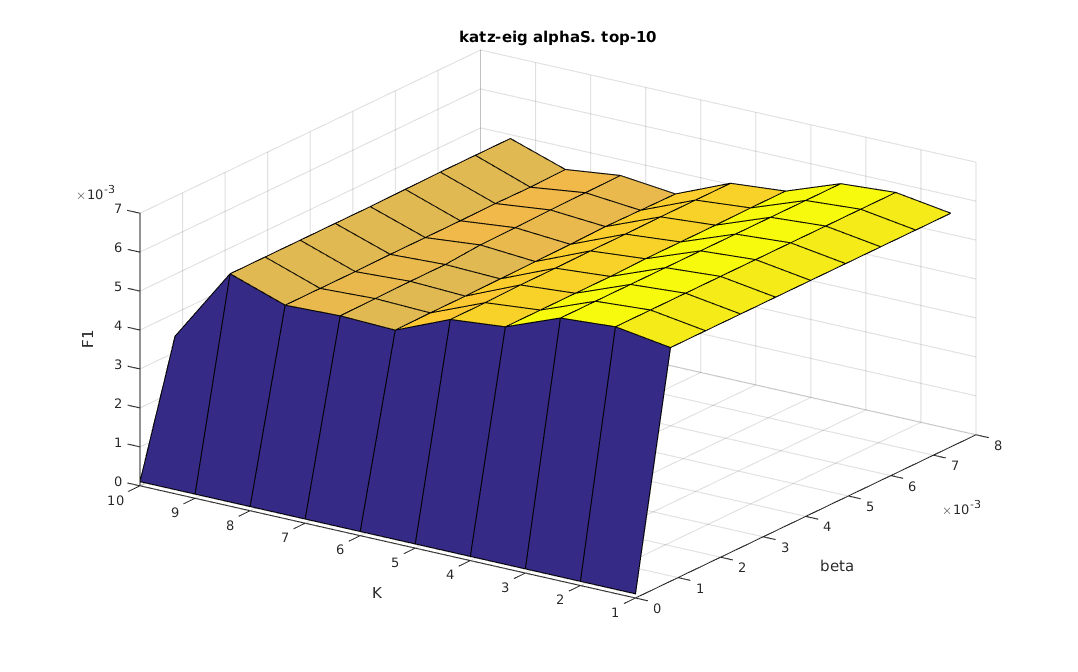
\includegraphics[width=\linewidth]{fig/katzeig_beta_k/alphaS_katzeig.png}
    \captionof{figure}{\textit{alphaS}}
\end{minipage}%
\begin{minipage}{.5\textwidth}
    \centering
    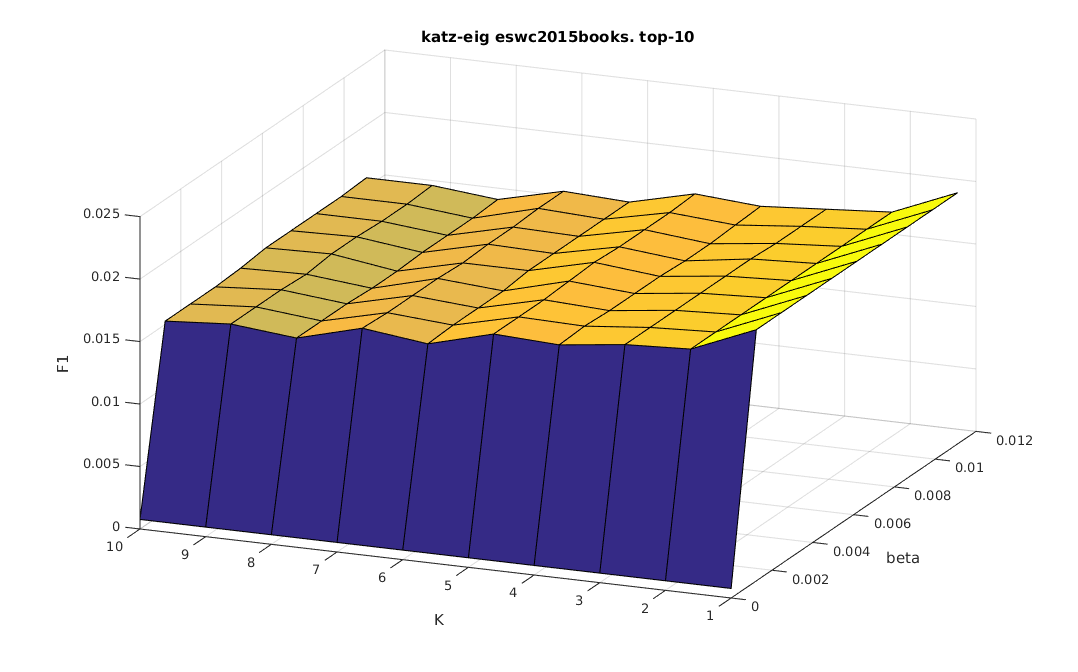
\includegraphics[width=\linewidth]{fig/katzeig_beta_k/eswc2015books_katzeig.png}
    \captionof{figure}{\textit{eswc2015books}}
\end{minipage}
\end{figure}

\begin{figure}[h!]
\centering
\begin{minipage}{.5\textwidth}
    \centering
    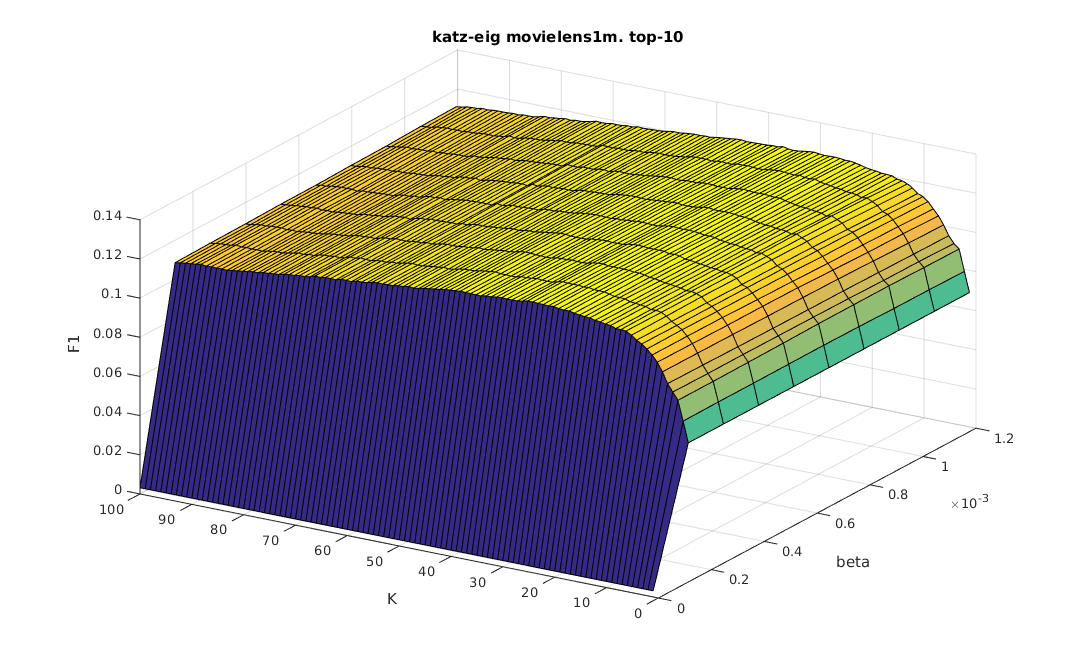
\includegraphics[width=\linewidth]{fig/katzeig_beta_k/movielens_katzeig.png}
    \captionof{figure}{\textit{movielens1m}}
\end{minipage}%
\begin{minipage}{.5\textwidth}
    \centering
    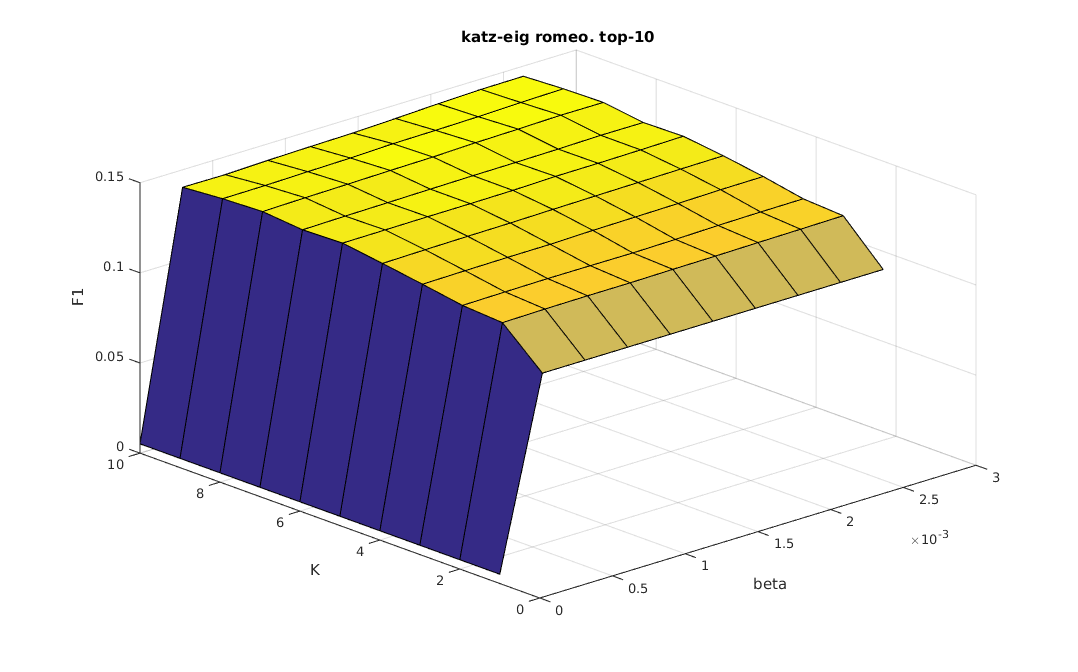
\includegraphics[width=\linewidth]{fig/katzeig_beta_k/romeo_katzeig.png}
    \captionof{figure}{\textit{romeo}}
\end{minipage}
\end{figure}




It seems like $beta$ doesn't have a very big impact on the function value. Some plots with a fixed $K$ follows to better see differences.

The range examined is $0 < \beta \leq \beta_{max} = \frac{1}{\|A_{train}\|_2}$ with a $K$ selected to fit the specific dataset. Again evaluated using \textit{Precision}, \textit{Recall} and \textit{F-measure} w.r.t. the test set using the top-10 recommendations.

\FloatBarrier

\begin{figure}[h!]
\centering
\begin{minipage}{.5\textwidth}
    \centering
    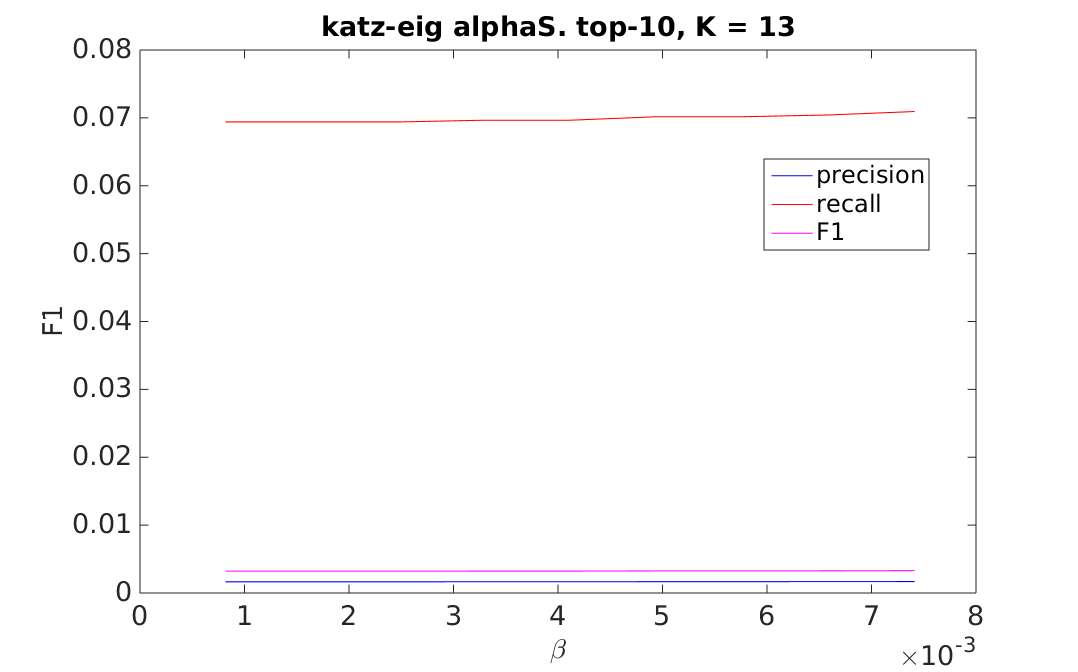
\includegraphics[width=\linewidth]{fig/katzeig_beta/alphaS_katzeig_beta.png}
    \captionof{figure}{\textit{alphaS}.
        $\beta_{max}$ is the best value with a $1.9\%$ diff between the minimum and the maximum \textit{F1} value.}
\end{minipage}%
\begin{minipage}{.5\textwidth}
    \centering
    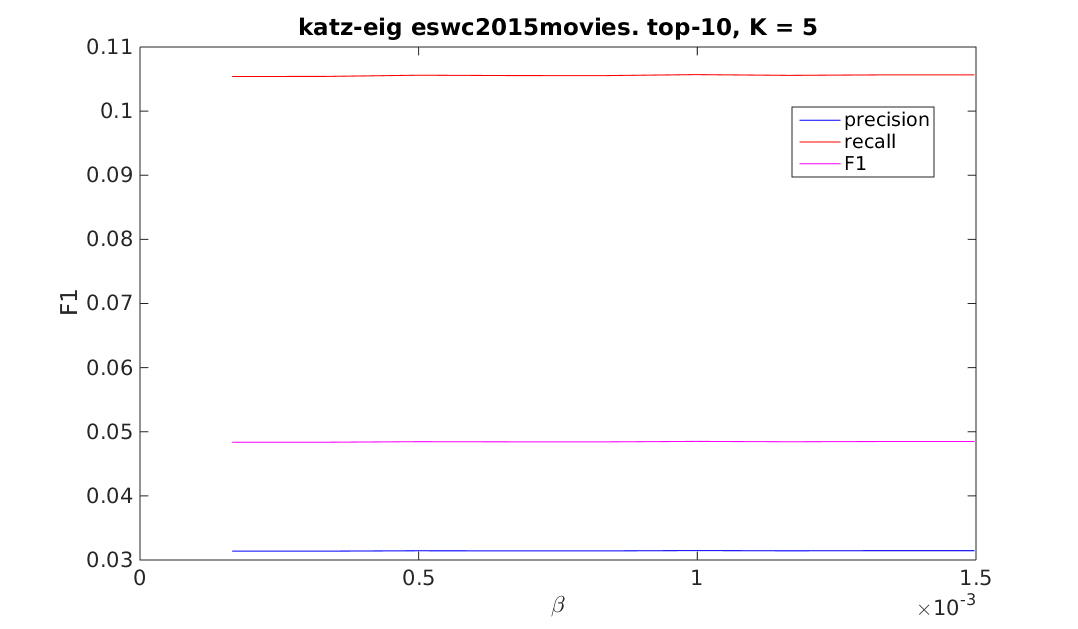
\includegraphics[width=\linewidth]{fig/katzeig_beta/eswc2015movies_katzeig_beta.png}
    \captionof{figure}{\textit{eswc2015movies}.
        $\beta_{max}$ is not the best value with a $0.3\%$ diff between the minimum and the maximum \textit{F1} value.}
\end{minipage}
\end{figure}

\begin{figure}[h!]
\centering
\begin{minipage}{.5\textwidth}
    \centering
    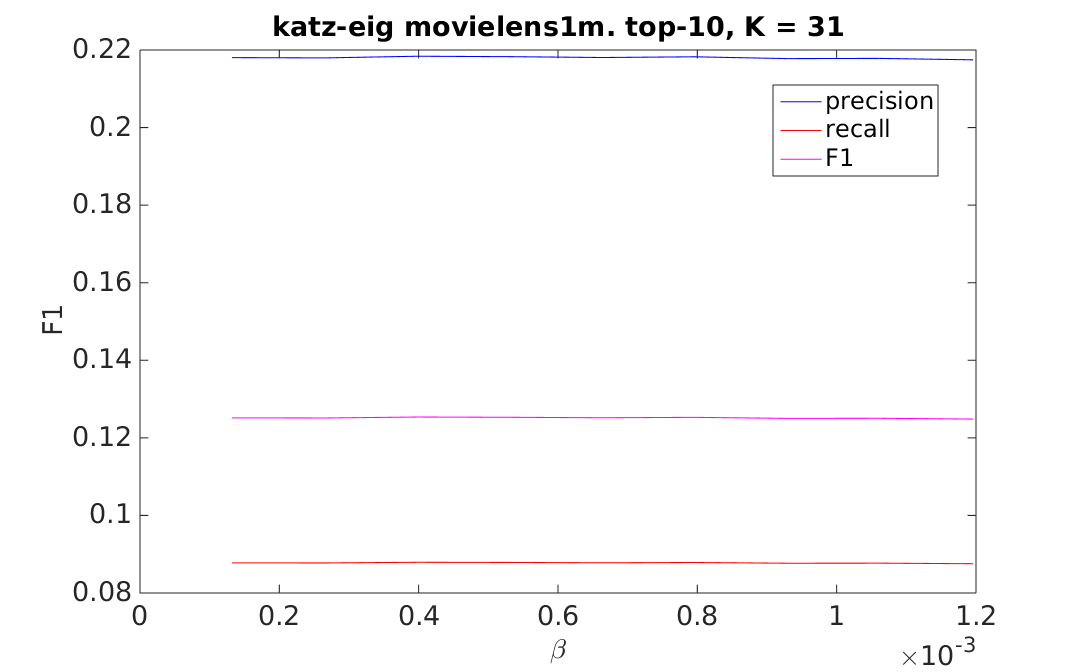
\includegraphics[width=\linewidth]{fig/katzeig_beta/movielens_katzeig_beta.png}
    \captionof{figure}{\textit{movielens1m}.
        $\beta_{max}$ is not the best value with a $0.41\%$ diff between the minimum and the maximum \textit{F1} value.}
\end{minipage}%
\begin{minipage}{.5\textwidth}
    \centering
    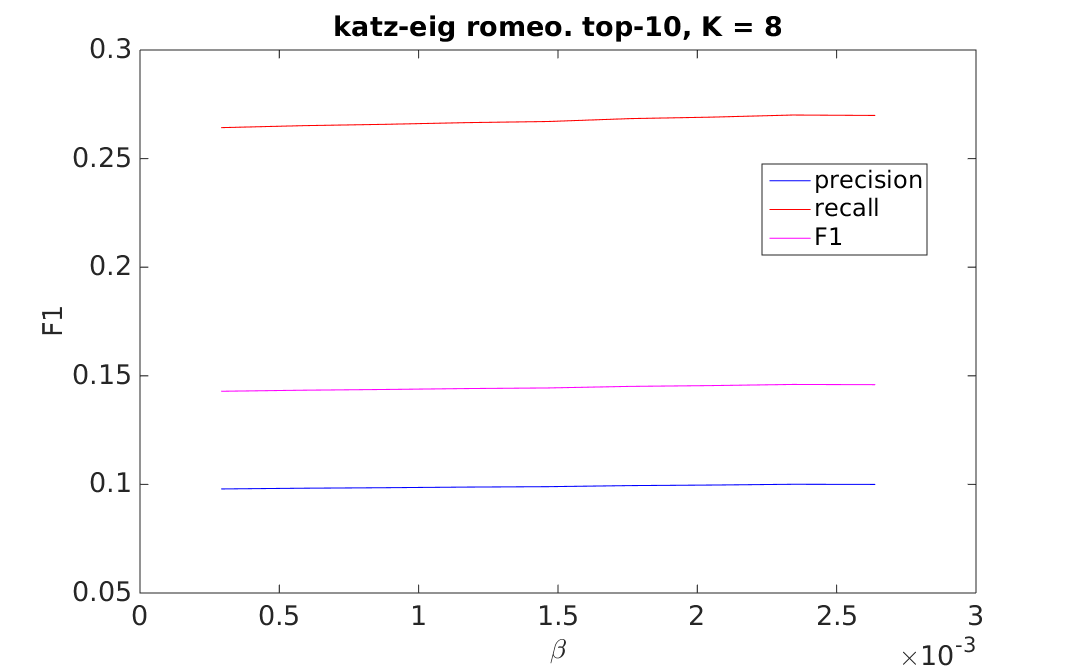
\includegraphics[width=\linewidth]{fig/katzeig_beta/romeo_katzeig_beta.png}
    \captionof{figure}{\textit{movielens1m}.
        $\beta_{max}$ is not the best value with a $2.09\%$ diff between the minimum and the maximum \textit{F1} value.}
\end{minipage}
\end{figure}

\FloatBarrier

The difference between the optimal $\beta$ and an arbitrary selected $\beta$ isn't very large. Even smaller is the difference between the optimal $\beta$ and $\beta_{max}$.  \Tableref{tab:katzeig_beta} is a summary of the evaluated values.

\begin{table}[h!]
    \centering
    \begin{tabular}{| c | r | r | r | r | l |}
        \hline
        \textbf{dataset}        & \textbf{diff between $\beta_{opt}$ and $\beta_{max}$ }    & \textbf{diff between $f_{min}$ and $f_{max}$} \\ \hline

        \textit{alphaS}         & 0~\%      & 2.0~\%    \\ \hline
        \textit{eswc2015books}  & 0~\%      & 0\%       \\ \hline
        \textit{eswc2015movies} & 0.039~\%  & 0.28~\%   \\ \hline
        \textit{movielens1m}    & 0.41~\%   & 0.41~\%   \\ \hline
        \textit{romeo}          & 0.072~\%  & 2.1~\%    \\ \hline


    \end{tabular}
    \caption{A summary of evaluating different $\beta$. $\beta_{max} = \frac{1}{\|A_{train}\|_2}$ is the maximally examined $\beta$ and $\beta_{opt}$ is the optimal $\beta$ found in the range $0 < \beta \leq \beta_{max}$. $K$ is individually optimized for the different datasets. $f_{min}$ and $f_{max}$ are the minimal and maximal \textit{F1} values obtained.}
    \label{tab:katzeig_beta}
\end{table}

\FloatBarrier

\newpage


The $K$-rank approximation represents different available models for \textit{katz-eig}. The following plots show different values of $K$, evaluated w.r.t. the test set. $\beta = \frac{1}{\|A_{train}\|}_2$ for all datasets. $K_{m}$ is the value of $K$ which gives the best \textit{F-measure} for each dataset.

\FloatBarrier

\begin{figure}[h!]
\centering
\begin{minipage}{.5\textwidth}
    \centering
    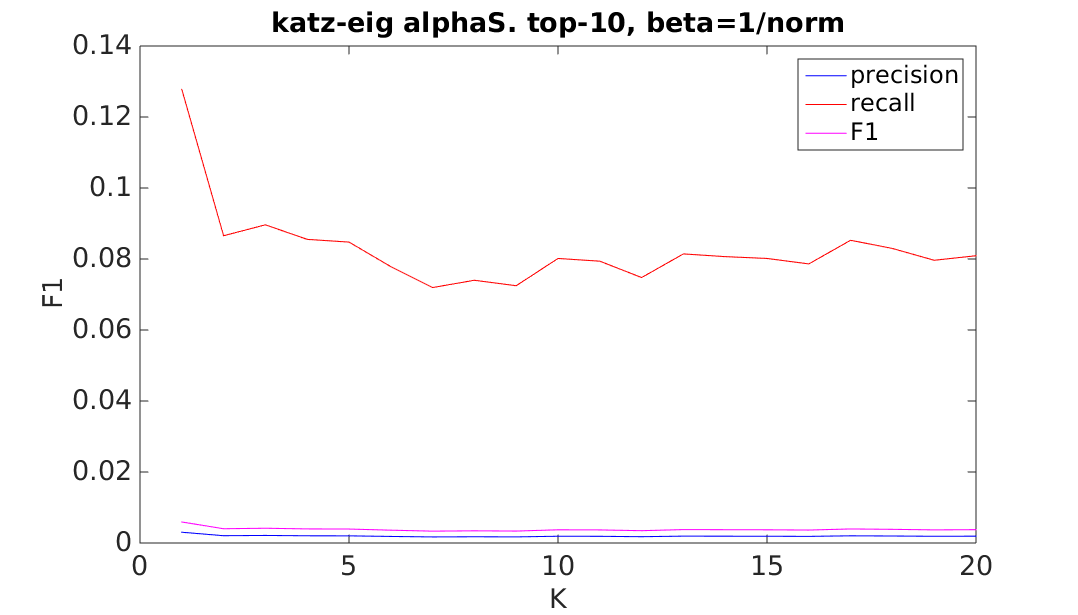
\includegraphics[width=\linewidth]{fig/katzeig_k/alphaS_katzeig_K.png}
    \captionof{figure}{\textit{alphaS} $K_{m} = 13$}
\end{minipage}%
\begin{minipage}{.5\textwidth}
    \centering
    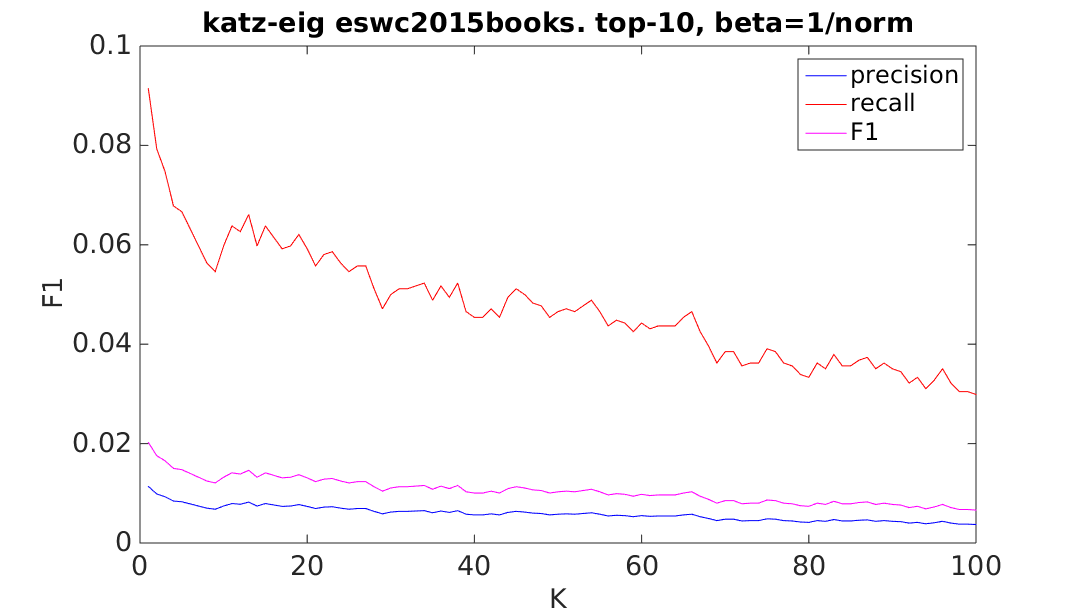
\includegraphics[width=\linewidth]{fig/katzeig_k/eswc2015books_katzeig_K.png}
    \captionof{figure}{\textit{eswc2015books} $K_{m} = 1$}
\end{minipage}
\end{figure}

\begin{figure}[h!]
\centering
\begin{minipage}{.5\textwidth}
    \centering
    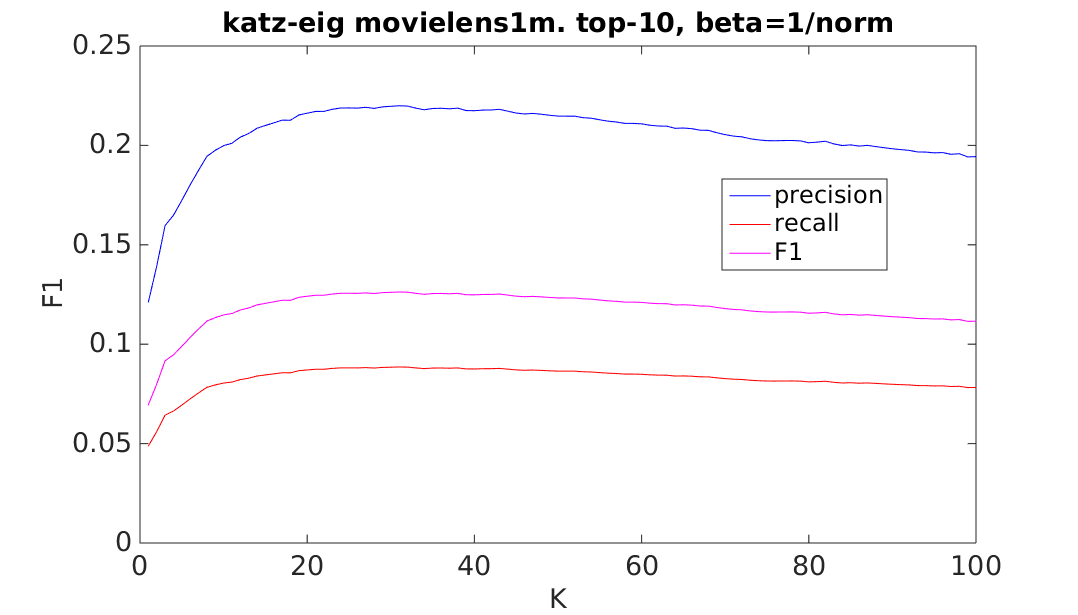
\includegraphics[width=\linewidth]{fig/katzeig_k/movielens_katzeig_K.png}
    \captionof{figure}{\textit{movielens1m} $K_{m} = 31$}
\end{minipage}%
\begin{minipage}{.5\textwidth}
    \centering
    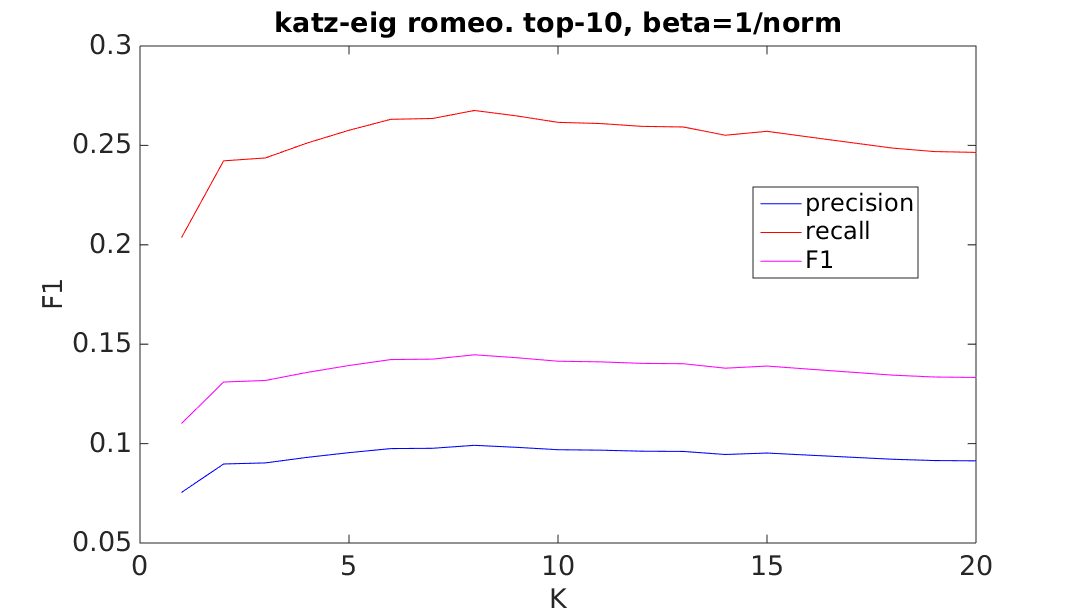
\includegraphics[width=\linewidth]{fig/katzeig_k/romeo_katzeig_K.png}
    \captionof{figure}{\textit{romeo} $K_{m} = 8$}
\end{minipage}
\end{figure}

\Warning[TODO]{ Plot of \textit{eswc2015movies}? }

%\begin{figure}[h!]
%\centering
%\begin{minipage}{.5\textwidth}
    %\centering
    %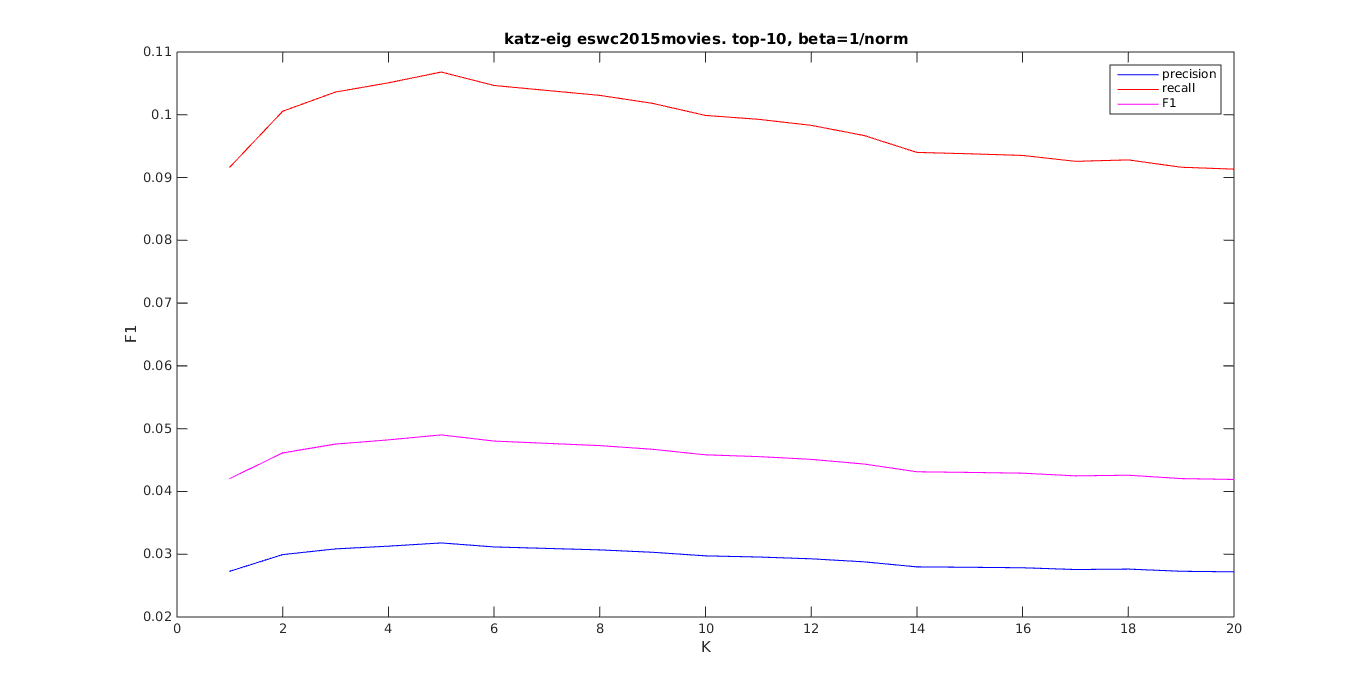
\includegraphics[width=\linewidth]{fig/katzeig_k/eswc2015movies_katzeig_K.png}
    %\captionof{figure}{\textit{eswc2015movies} $K_{m} = 5$}
%\end{minipage}%
%\begin{minipage}{.5\textwidth}
    %\centering
    %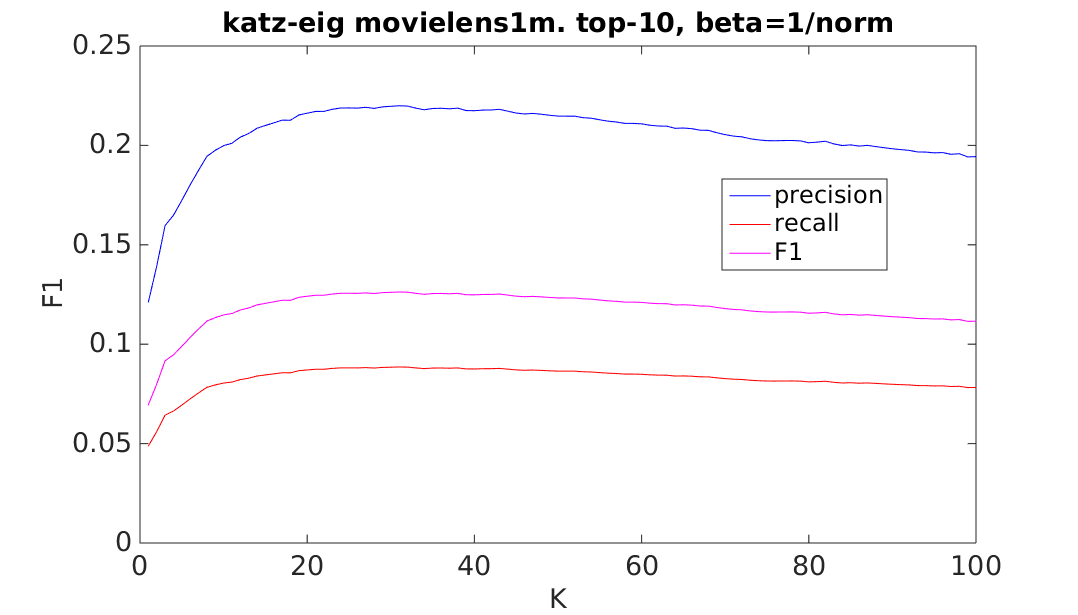
\includegraphics[width=\linewidth]{fig/katzeig_k/movielens_katzeig_K.png}
    %\captionof{figure}{\textit{movielens1m} $K_{m} = 31$}
%\end{minipage}
%\end{figure}

%\begin{figure}[h!]
%%\centering
%\begin{minipage}{.5\textwidth}
    %%\centering
    %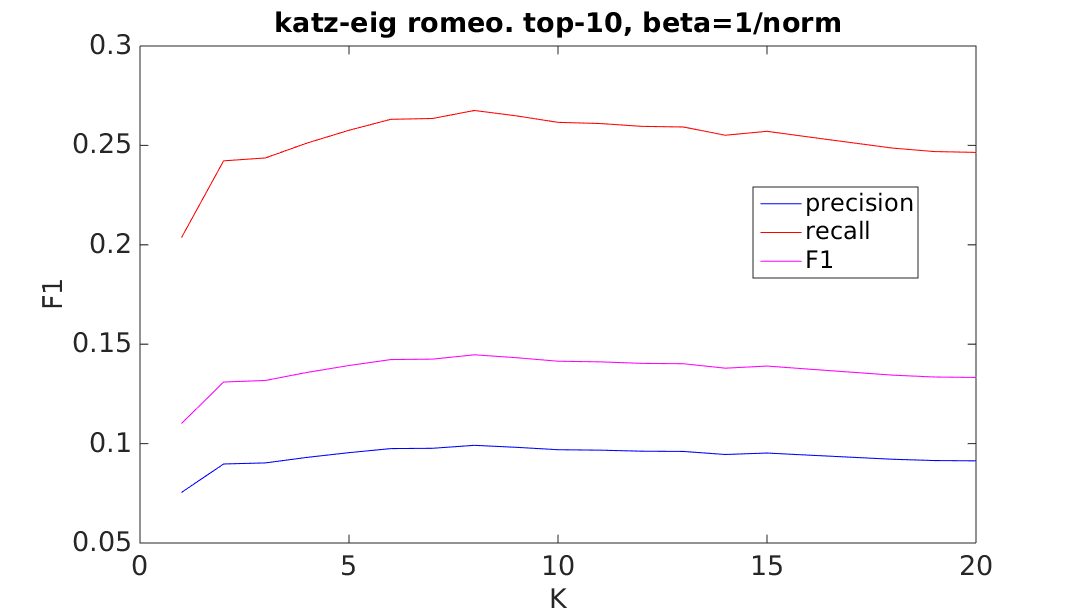
\includegraphics[width=\linewidth]{fig/katzeig_k/romeo_katzeig_K.png}
    %\captionof{figure}{\textit{romeo} $K_{m} = 8$}
%\end{minipage}%
%\end{figure}

\FloatBarrier

The function space w.r.t. $K$ is fairly smooth if not entirely convex. \textit{eswc2015books} is an outlier with a low optimal value $K = 1$ and many local optima. The other datasets display more smooth functions, but there are clear local optima with both \textit{alphaS} and \textit{romeo}.

Also of note is that the functions start to decline at different $K$. \textit{eswc2015movies} declines already at $K = 5$ but it's only at around $K = 30$ \textit{movielens1m} starts to decline. As noted earlier \textit{eswc2015books} has it's optima already at $K = 1$.


%\newpage

%\section{The link-analysis algorithm}\label{sec:linkanalysis}

%\textit{Cleanup, mostly description from article. Reduce information?}

The \textit{link-analysis} algorithm, as presented by \cite{huang2004link} and further discussed in \cite{huang2007comparison}. See the articles for more information and in-depth examples. What follows is a condensed description of how the algorithm works.

The algorithm is an adaptation of HITS \cite{kleinberg1999authoritative} which is a web page ranking algorithm to the recommendation domain. The original algorithm distinguish between \textit{Authoritative} pages which definitely contain high-quality information and \textit{Hub} pages which are comprehensive lists of links to authoritative pages. \citep{huang2007comparison}

The adaptation to the recommendation domain is achieved by introducing the \textit{product representativeness} score $\PR$ and the \textit{consumer representativeness} score $\CR$.

The \textit{product representativeness} score $\PR(i, u)$ can be seen as a measure of the item $i$'s level of interest with respect to user $u$, or in other words $i$'s authority of $u$'s interests in $i$.

The \textit{consumer representativeness} score $\CR(u, \hat{u})$ measures how well $u$ as a hub for $\hat{u}$ associates with products of interests to $\hat{u}$.

If $h_{u, i}$ is the user-item interaction history as defined by \ref{eq:hist} and $h$ is the interaction matrix then a recursive definition of the authority and hub scores can be defined as

\begin{equation}
    \PR = h' * \CR
\end{equation}

\begin{equation}
    \CR = B * \PR + \CR_0
\end{equation}

Where $B$ is a matrix such that:

\begin{equation}
    B_{u, i} = \frac{ h_{u, i} }{ \left(\sum_{i} h_{u, i}\right)^\gamma }
\end{equation}

Meaning $B$ normalizes the representativeness score a costumer receives from linked products by dividing it with the total number of products the customer is linked to.  $\gamma$ controls the extent to which a consumer is penalized for making many purchases.

$\CR_0$ is defined as

\begin{equation}
    \CR_{i, j}^0 = \begin{cases}
        \eta \quad \text{if } \; i = j \\
        0    \quad \text{otherwise}
    \end{cases}
\end{equation}

in other words $\CR_0 = \eta * I_M$ where $I_M$ is an $M x M$ identity matrix and $M$ is the number of users.  It is included to maintain the high representativeness score for the target users themselves. This also necessitates a normalization step to keep the values on a consistent level.

In summary the \textit{link-analysis} algorithm follow these steps:

\begin{enumerate}
    \item Construct the interaction matrix $A$ and the associating matrix $B$.

    \item Set $\CR_0 = \eta * I_M$.
    \item At each iteration $t = 1, \ldots, t_{max}$ perform:

        \begin{enumerate}
            \item $\PR_t = h' * \CR_{t- 1}$
            \item $\CR_t = B * \PR_t$
            \item Normalize $\CR_t$ so each column adds up to 1
            \item $\CR_t = \CR_t + \CR_0$
        \end{enumerate}

        Repeat until convergence.

    \item Predicted user-item interaction is given by $\mathit{pval} = \PR'$.

\end{enumerate}

There are two parameters to the algorithm: $\gamma$ and $\eta$.
%\Warning[TODO]{ Describe them, what's their purpose }


%\newpage





%\textit{Unsure about the rest!}

%\section{Big comparisons?}
%\Warning[TODO]{ title? Where? What? How? :) }

%Compare katz-eig, link-analysis, and some other algorithm?
%Also compare optimization w.r.t. time and evaluation.

%\begin{enumerate}
    %\item Running time
    %\item F-measure
%\end{enumerate}


%\section{Optimization}\label{sec:res:opt}

%Optimization techniques in broad stroaks.

%Resulting graphs from LinkAnalysis. Use different kinds of datasets.

%\begin{itemize}
    %\item Graph over $\gamma$ with fixed $\eta$.
    %\item Graph over $\eta$ with fixed $\gamma$.
    %\item Graph over $\gamma$, $\eta$.
    %\item Graph over $T$, see that things flattens out.
%\end{itemize}

%Similarly for KatzEig.


%Compare custom\_neighbour, custom\_neighbour\_step, fminsearch, ... with each other. Compare runtime and accuracy over different kinds of datasets.

%Similarly for KatzEig.



%\subsection{Julia}\label{subsec:res:julia}

%\Warning[TODO]{ Move to discussion? Conclusions? }

%Although not a focus of this thesis, some explorations with Julia has been undertaken.


